\documentclass[journal]{IEEEtran}

% *** PACKAGES ***
\usepackage{cite}          % For citations
\usepackage{amsmath}       % For math symbols and equations
\usepackage{amsfonts}      % For math fonts
\usepackage{graphicx}      % For including graphics
\usepackage{algorithmic}   % For algorithms
\usepackage{array}         % For tables
\usepackage{url}           % For URLs
\usepackage{float} % for the [H] placement specifier

% *** TITLE AND AUTHORS ***
\title{Predição de Estabilidade para Smart Grid}
\author{Victor Jorge Carvalho Chaves 159740,
        João Vinicius Farah Colombini 159501}

% *** BEGIN DOCUMENT ***
\begin{document}

\maketitle

%%% Faz o resumo
\begin{abstract}
    Com o crescimento do consumo de energia elétrica pelo mundo, é essencial garantir sua disponibilidade e monitoramento, e para isso, é proposto um trabalho que vá prever o estado de uma rede elétrica.
\end{abstract}

\begin{IEEEkeywords}
    Rede Elétricas Inteligentes, Aprendizado de Máquina
\end{IEEEkeywords}

\IEEEpeerreviewmaketitle

\section{Introdução}
As redes elétricas modernas enfrentam desafios crescentes de estabilidade e confiabilidade devido à integração de fontes de energia renováveis e à complexidade das demandas de carga. Neste contexto, este projeto propõe a aplicação de algoritmos de aprendizado de máquina, especificamente técnicas de regressão em aprendizado supervisionado, para estimar com precisão a estabilidade desses sistemas elétricos. Ao utilizar métodos avançados de regressão, busca-se desenvolver modelos capazes de prever valores contínuos que representam indicadores críticos de estabilidade.

Além do uso de regressão é muito eficaz procurar uma série de parâmetros para descrever o funcionamento desses sistemas elétricos e para  isso, após uma análise com regressão, também é implementado um Algoritmo Genético para tentar solucionar esse problema.

\section{Contexto}

Na área de desenvolvimento de soluções inteligentes para aprendizado sobre o comportamento de redes elétricas inteligentes (Smart Grid), foi desenvolvido uma base de dados simulada$^{[8]}$ de uma rede elétrica controlada de forma descentralizada.

A partir desse trabalho, foi realizado diversos trabalhos cientificos utilizando destes dados, todas com foco em resolver tarefas de classificação da estabilidade da rede.

Com isso, este estudo tem como objetivo achar uma solução que resolva a tarefa de regressão da estabilidade da rede.

As váriaveis que há nessa base são as seguintes:

\begin{itemize}
    \item \texttt{tau[x]}: Tempo de reação do participante (valor real no intervalo [0.5, 10] segundos).
          \begin{itemize}
              \item \texttt{tau1} - valor para o produtor de eletricidade;
          \end{itemize}
    \item \texttt{p[x]}: Potência nominal consumida (negativa) ou produzida (positiva) (valor real).
          \begin{itemize}
              \item Para consumidores, no intervalo [-0.5, -2] segundos$^{-2}$;
              \item \texttt{p1} = abs(\texttt{p2} + \texttt{p3} + \texttt{p4});
          \end{itemize}
    \item \texttt{g[x]}: Coeficiente $(\gamma)$ proporcional à elasticidade de preço (valor real no intervalo [0.05, 1] segundos$^{-1}$).
          \begin{itemize}
              \item \texttt{g1} - valor para o produtor de eletricidade;
          \end{itemize}
    \item \texttt{stab}: A parte real máxima da raiz da equação característica (se positiva - o sistema é linearmente instável) (valor real).
    \item \texttt{stabf}: A classificação de estabilidade do sistema (categórica: estável/instável).
\end{itemize}


\section{Metodologia}
\subsection{Principais Técnologias}

As principais bibliotecas utilizadas foram:
\begin{itemize}
    \item Pandas: Manipulação e análise de dados
    \item Numpy: Manipulação e análise de dados
    \item MatplotLib: Visualização
    \item seaborn: Visualização
    \item sklearn: Biblioteca de aprendizado de máquina
    \item lightgbm: Modelo de aprendizado de máquina utilizando o método
    \item xgboost
    \item PyGAD: Algoritmo Genético
    \item Torch: Para implementação de CUDA
\end{itemize}

\subsection{Extração dos dados}

Os dados foram extraídos do Repositório de Aprendizado de Máquina da UC Irvine.

\subsection{Análise na Correlação entre as váriaveis}

Para análise da correlação em relação ao banco de dados, o método utilizado foi o de correlação de pearson que varia de $-1$ a $1$ Sendo que $1$ é correlação positiva forte e $-1$ é correlação negativa forte, $0$ corresponde a zero correlação.

Para apresentar de maneira gráfica foi utilizado um mapa de calor que deixa evidente os maiores e menores valores.


\subsection{Competição entre os Modelos de regressão}

Para esse projeto foram utilizados 18 métodos para regressão, dos mais básicos aos mais avançados, como os que usam boosting de gradiente ou AdaBoosting.

Entre eles:

\begin{itemize}
    \item {Bayesian Ridge Regression}
    \item {Automatic Relevance Determination (ARD) Regression}
    \item {Lasso Regression}
    \item {Ridge Regression}
    \item {Linear Regression}
    \item {Support Vector Regression (SVR)}
    \item {Nu Support Vector Regression (NuSVR)}
    \item {Light Gradient Boosting Machine (LGBM)}
    \item {k-Nearest Neighbors Regression (KNN)}
    \item {Elastic Net Regression}
    \item {AdaBoost Regression}
    \item {Stochastic Gradient Descent Regression (SGD)}
    \item {Extra Trees Regression}
    \item {eXtreme Gradient Boosting (XGBoost)}
    \item {Multi-layer Perceptron Regression (MLP)}
    \item {Random Forest Regression}
    \item {Histogram-based Gradient Boosting Regression}
    \item {Gradient Boosting Regression}
    \item {Decision Tree Regression}
\end{itemize}

Para avalia-los os métodos utilizados em K-folds foram:

\begin{itemize}
    \item Erro Absoluto Médio (MAE)
    \item Erro Quadrático Médio (MSE)
    \item Erro Percentual Absoluto Médio (MAPE)
    \item Coeficiente de Determinação (R²)
\end{itemize}

E portanto ao avaliar isso foram separados 3 modelos principais:

\begin{itemize}
    \item {Nu Support Vector Regression (NuSVR)}
    \item {Light Gradient Boosting Machine (LGBM)}
    \item {Histogram-based Gradient Boosting Regression}
\end{itemize}

Nu Support Vector Regression é um tipo de regressão por SVM, que utiliza de um parâmetro Nu que é utilizado como dois limites, o limite superior representa o número de vetores de suporte e como um limite inferior para os pontos dentro da margem.

Light Gradient Boosting Machine, utiliza de combinações referentes a vários modelos individuais nesse caso com árvores de decisão para regressão e posteriormente combina vários desses modelos mais "fracos" e forma um modelo  com resultados mais significativos (ou "Fortes").

Histogram-based Gradient Boosting Regression Utiliza a mesma ideia de conceito de boosting de gradiente, mas utilizando histogramas.
Isso ocorre da seguinte maneira, ao invés de gerar splits diretamente nos nós das árvores de decisão eles formam bins que são intervalos (assim como em um histograma) e portanto isso simplifica o processo de gerar splits melhores.

\subsection{Filtragem dos modelos}

E a partir desses resultados, foi escolhido os três melhores modelos:



Com esses três modelos, foi aplicado a técnica de pesquisa em grade (Grid Search) para encontrar os melhores parâmetros em cada um desses modelos, e assim verificar os melhores resultados.

\subsection{Criação de um modelo de com Algoritmo genético}

A ideia principal desse tópico é gerar uma função que dados os parâmetros $x_1,x_2,...,x_n$ onde $n = 12$, tenham constantes $\lambda_1,\lambda_2,...,\lambda_n$, que multiplicando esses parâmetros cheguem a um resultado dizendo se aquele sistema elétrico é estável ou instavel.

Para isso foram utilizados os parâmetros de:
\begin{itemize}
    \item Número de gerações;
    \item Número de soluções a serem selecionadas para cruzamento;
    \item Soluções por população;
    \item Porcentagem de Mutação;
    \item Número de genes.
\end{itemize}

Esses parâmetros impactam diretamente no Fitness dessas equações.

Fitness ->

Além disso na biblioteca PyGAD tem dois jeitos de realizar o treinamento:
\begin{enumerate}
    \item Utiliza-se uma equação e um resultado, porém esse modelo foi utilizado com multiplas entradas e apenas um fitness para todas elas;
    \item E o método para multivariáveis, mas fica extremamente pesado carregar 8000 equações e 8000 fitness por geração.
\end{enumerate}

E para finalizar foram utilizados métodos para verificação da precisão que esse algoritmo gera.
\begin{enumerate}
    \item K-fold: Para garantir uma diferença nos resultados e um resultado final melhor e sem overfitting
    \item Resumir resultados finais em positivo ou negativo, como por exemplo: $y\_real = 0,0023$ e $y\_pred = 0.04$, os dois seriam iguais pois a ideia é verificar se o número é positivo ou negativo. (Isso foi utilizado pois fica impossivel chegar a um valor muito semelhante para um número muito grande de equações).
    \item Fazer cálculos com métricas de erro calcular o erro absoluto e relativo.
\end{enumerate}

\section{Resultados}
\subsection{Regressão}
Um dos primeiros resultados foi o mapa de calor com as correlações entre as variáveis como apresentado na Figura \ref{fig:heatMapCorr}.

\begin{figure}[H]
    \centering
    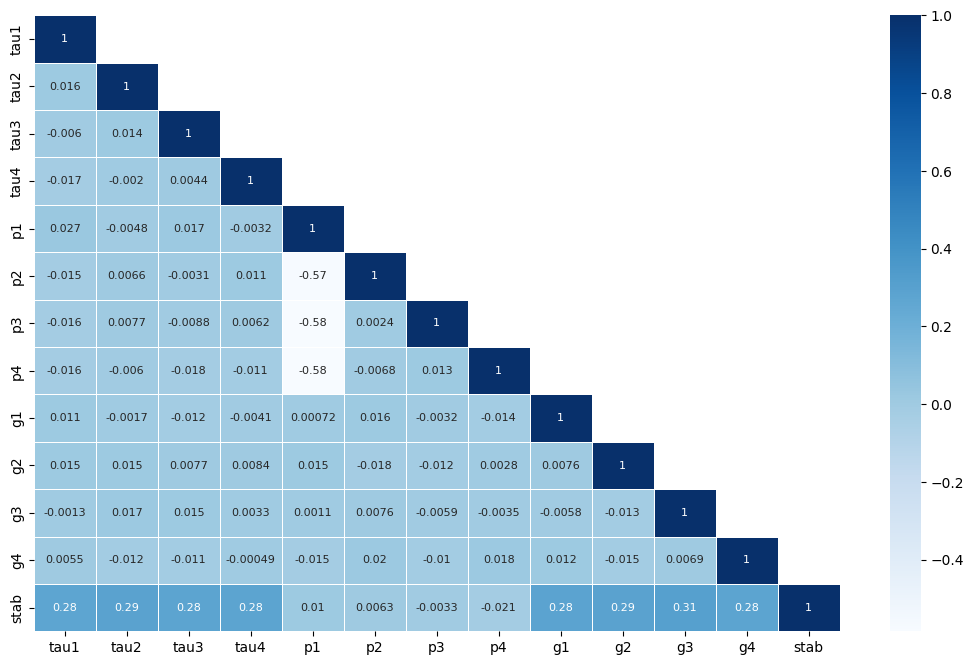
\includegraphics[width=1\linewidth]{Mapa_calor_corr.png}
    \caption{Mapa de calor - Correlações}
    \label{fig:heatMapCorr}
\end{figure}

Nele ficaram visiveis algumas variaveis com correlação fraca, mas pelo menos apresentam algum tipo de correlação. Fora isso é notável que os g's tem correlação com stab, portanto foi criada uma nova coluna também com as médias de g e ela apresentou a maior correlação positiva com stab que foi de aproximadamente $0.54$.%Não lembro o valor direito, corrigir?

Com base nesses dados os p's não pareciam tão relevantes, pois a busca era por uma correlação positiva forte, o que gerou uma série de dúvidas e algumas decisões como remover ou não os p's para fazer alguma regressão.

Após o tratamento dos dados, como eram simulados não havia a necessidade de preencher neutros nem algo do tipo. Inicia-se a etapa de avaliação de modelos para regressão baseados nesses dados.

Em relação a aqueles $18$ modloes foram obtidos os seguintes resultados referentes a $R^2$ e MAE, MSE, RMSE. (Representadas pelas Figuras \ref{fig:MAE18}, \ref{fig:MSE18}, \ref{fig:MAPE18}, \ref{fig:R218}).

\begin{figure}[H]
    \centering
    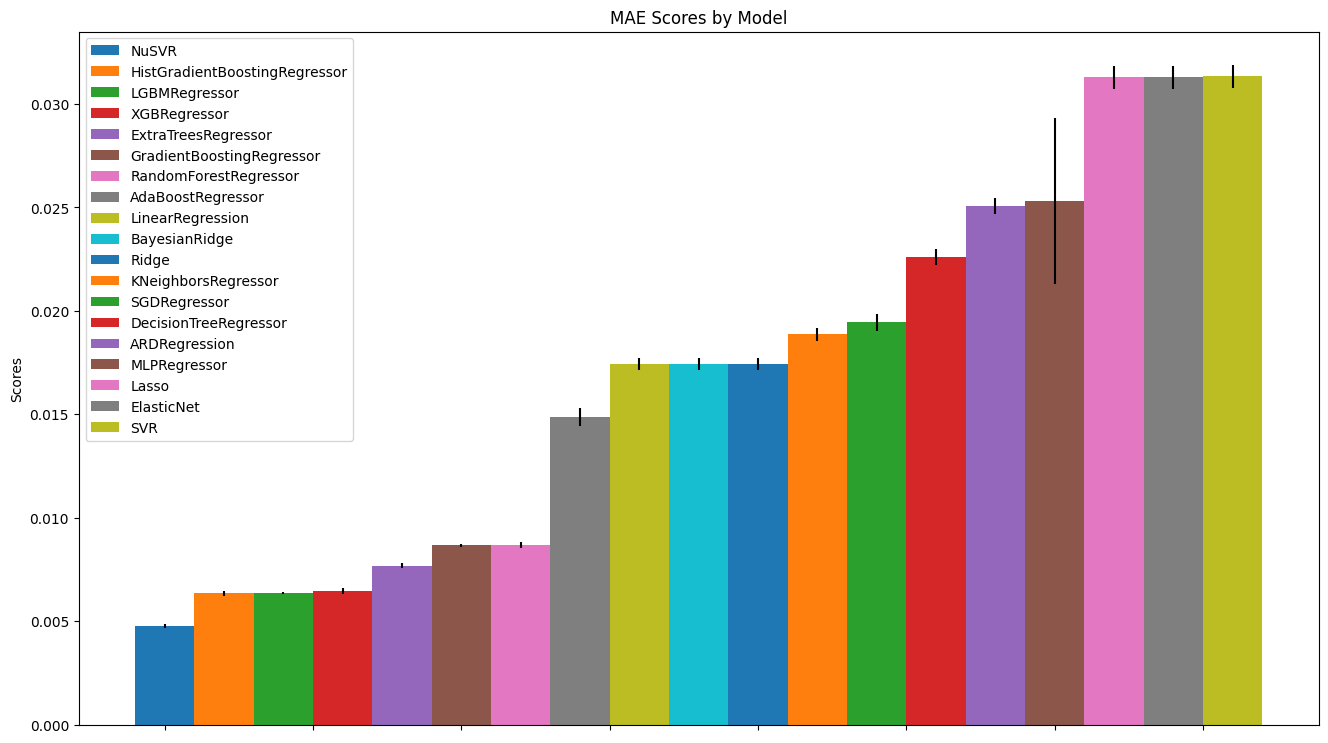
\includegraphics[width=1\linewidth]{image.png}
    \caption{Resultado MAE dos 18 modelos}
    \label{fig:MAE18}
\end{figure}


\begin{figure}[H]
    \centering
    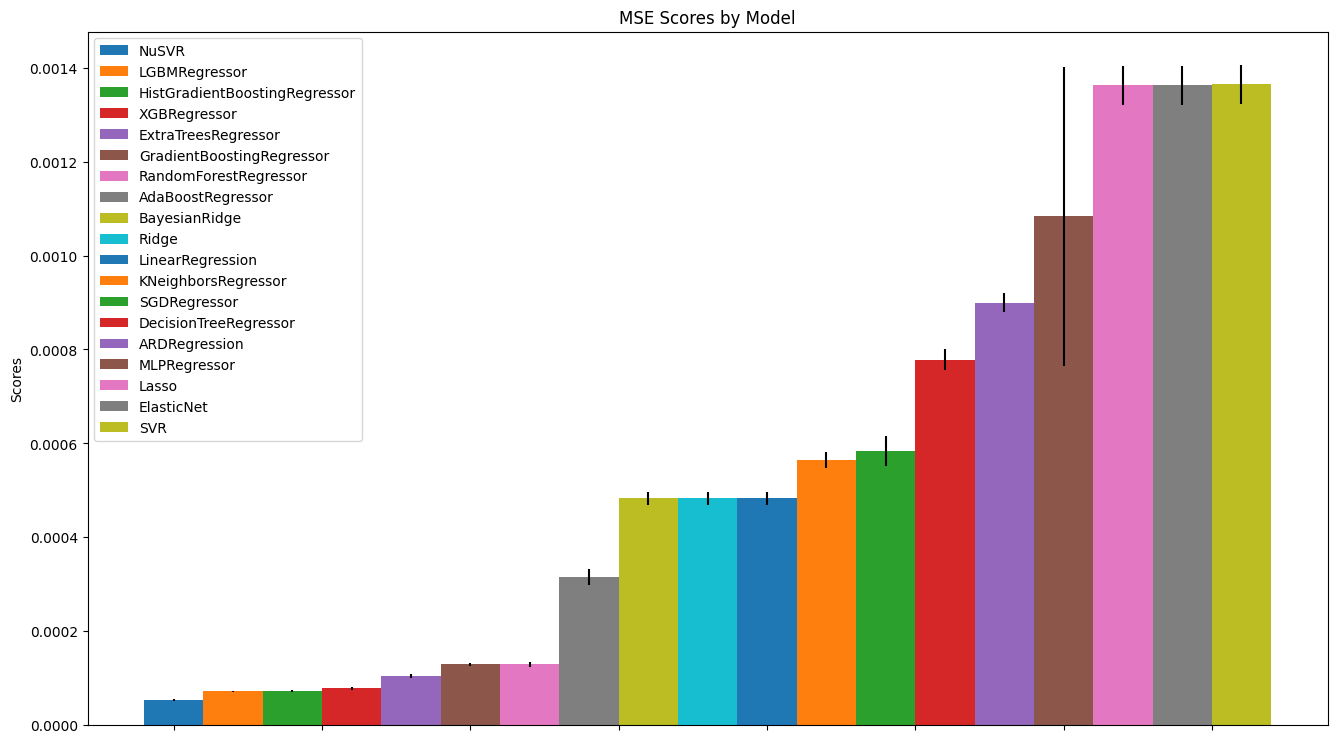
\includegraphics[width=1\linewidth]{image3.png}
    \caption{Resultado MSE dos 18 modelos}
    \label{fig:MSE18}
\end{figure}

\begin{figure}[H]
    \centering
    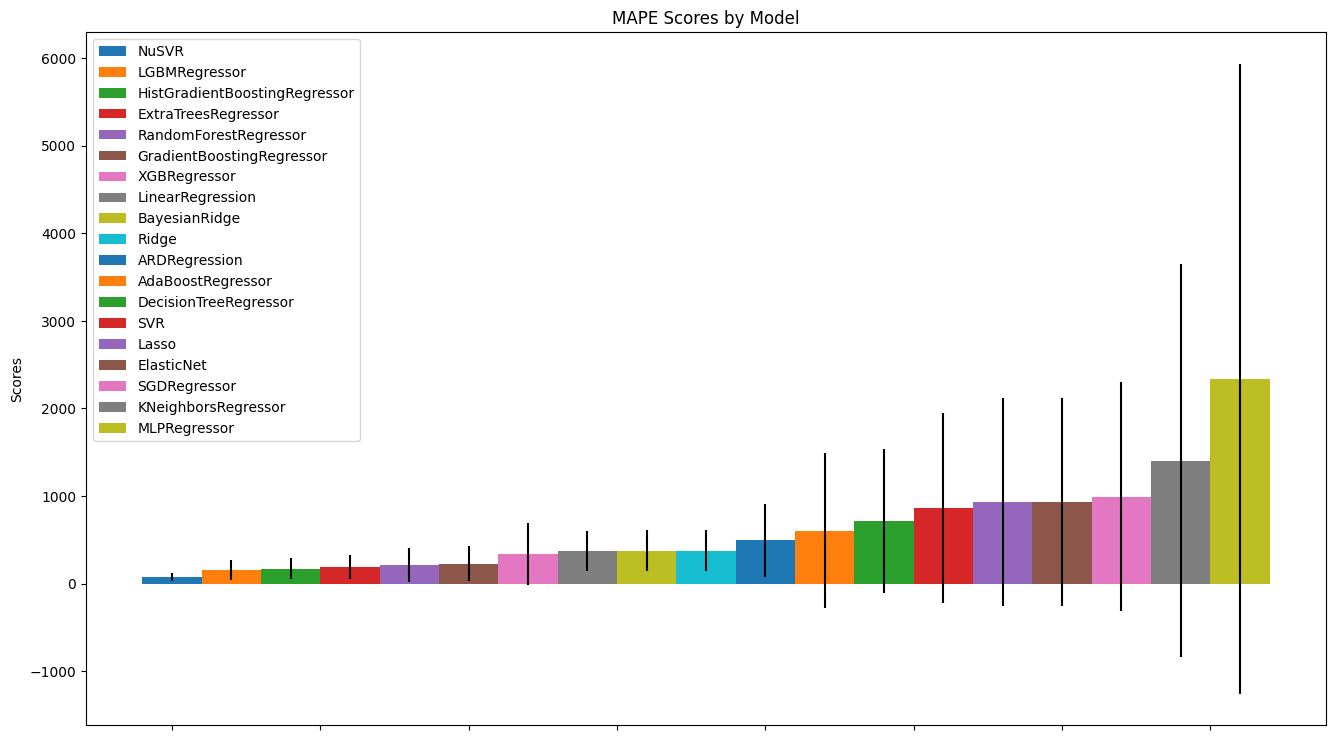
\includegraphics[width=1\linewidth]{image4.png}
    \caption{Resultado MAPE dos 18 modelos}
    \label{fig:MAPE18}
\end{figure}

\begin{figure}[H]
    \centering
    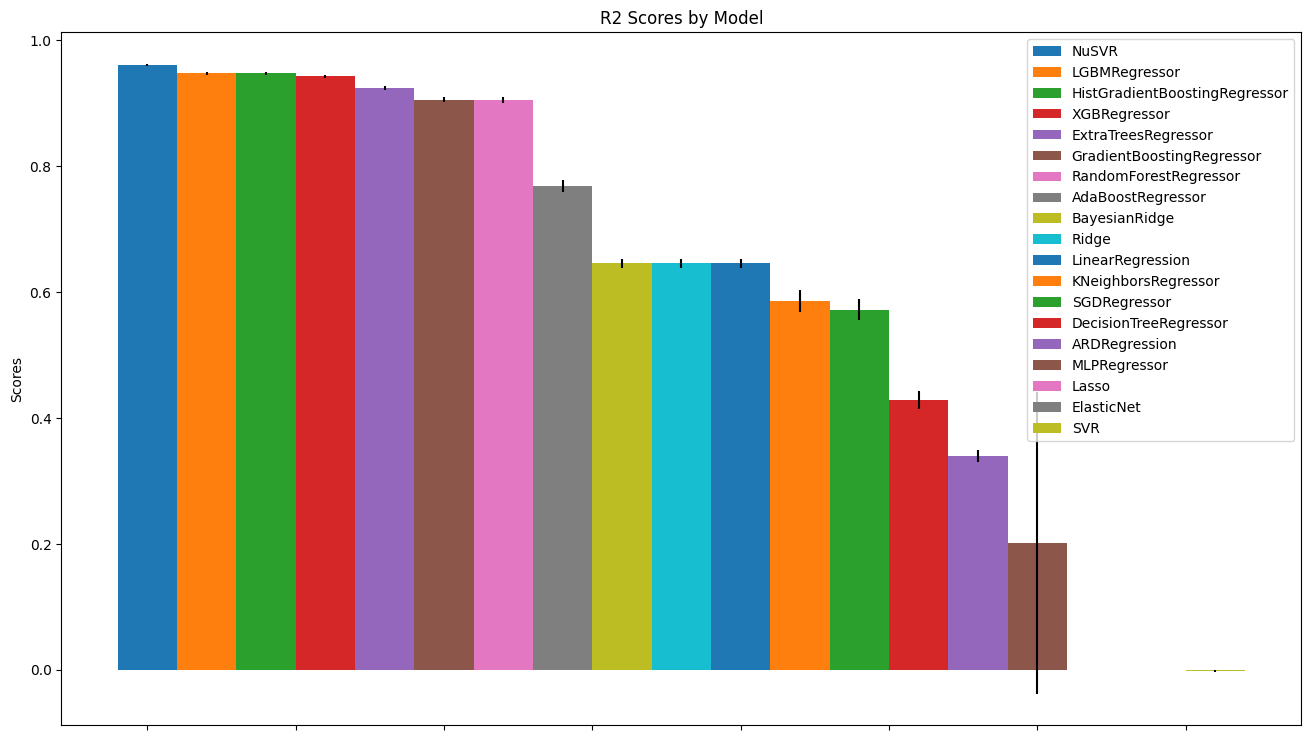
\includegraphics[width=1\linewidth]{image2.png}
    \caption{Resultado R2 dos 18 Modelo}
    \label{fig:R218}
\end{figure}



E após isso é simples a visualização de quais escolher, e portanto fazer uma avaliação mais aprofundada.

Como já dito e visualizado os mais performáticos foram: NuSVR, LighGBM e HistGradientBoosting.

Portanto foi preciso criar gráficos para verificar suas diferenças em um grau mais preciso e posteriormente decidir qual o melhor modelo a ser utilizado.

\begin{figure}[H]
    \centering
    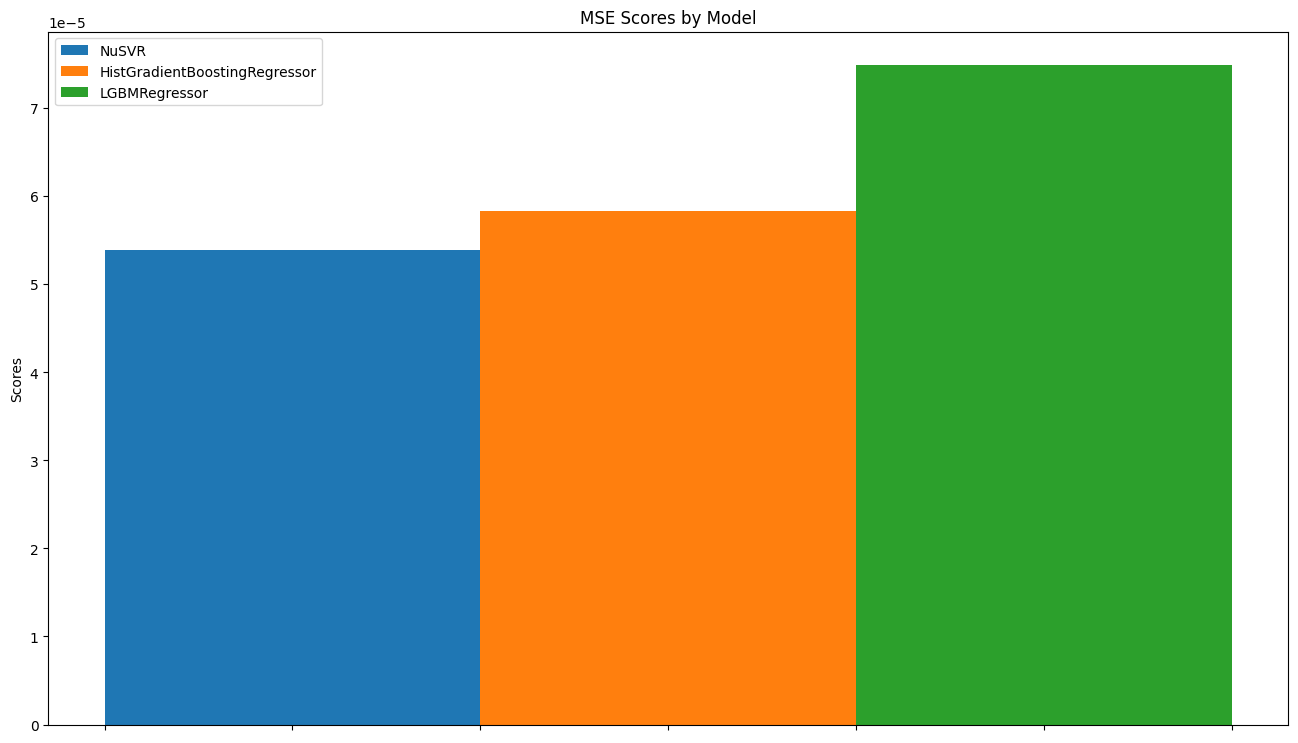
\includegraphics[width=1\linewidth]{7.png}
    \caption{MSE dos Modelos escolhidos}
\end{figure}

\begin{figure}[H]
    \centering
    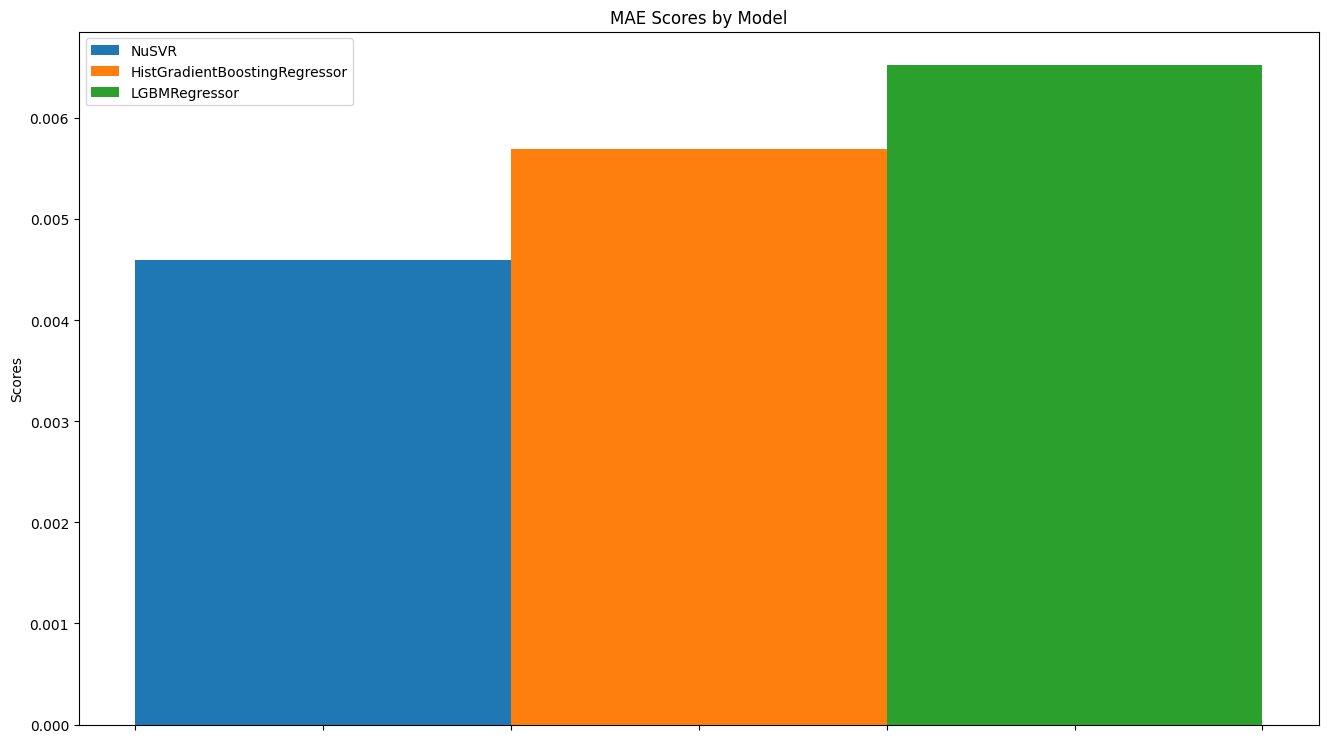
\includegraphics[width=1\linewidth]{9.png}
    \caption{MAPE dos modelos escolhidos}
\end{figure}

\begin{figure}[H]
    \centering
    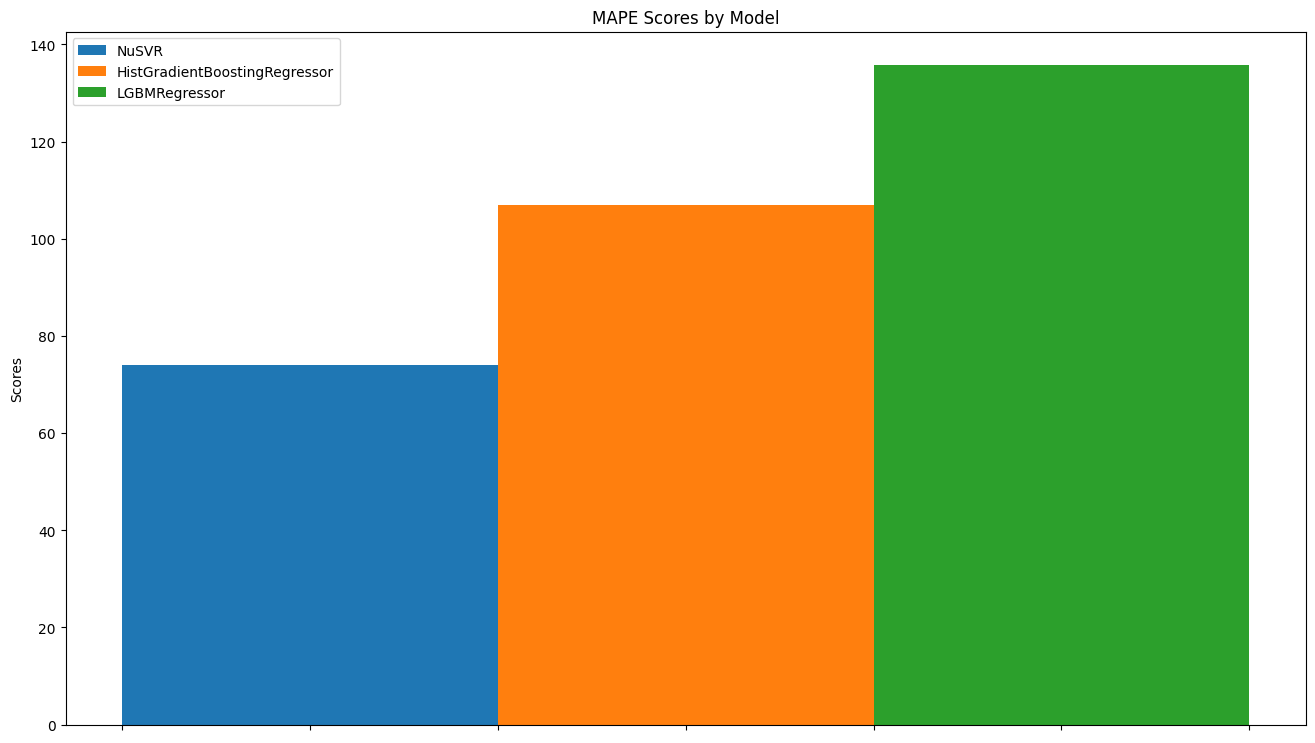
\includegraphics[width=1\linewidth]{10.png}
    \caption{MAE dos modelos escolhidos}
\end{figure}
\begin{figure}[H]
    \centering
    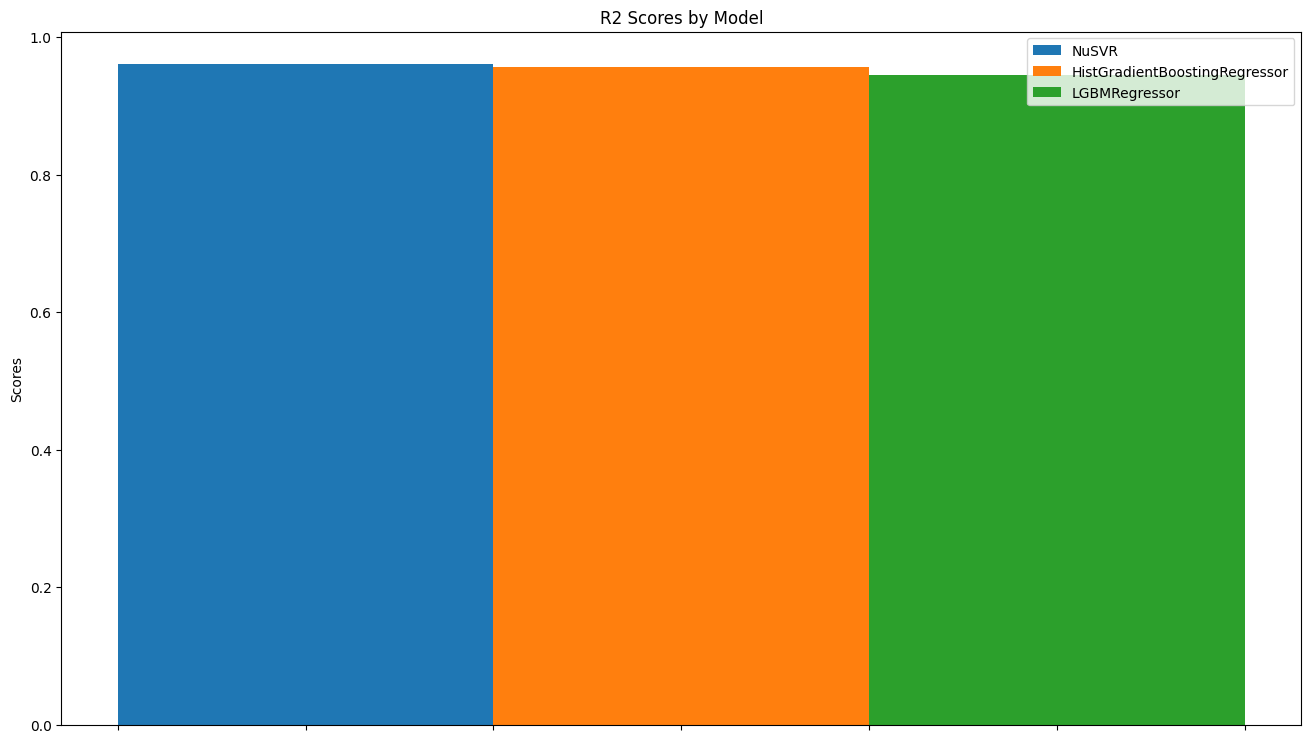
\includegraphics[width=1\linewidth]{12.png}
    \caption{R² dos modelos escolhidos}
\end{figure}

E por final também foram criadas visualizações das funções para utilizar da navalha de Occam (ou Ockham) para decidir qual o melhor modelo. (Representadas nas Figuras \ref{fig:LGBM_Func}, \ref{fig:NuSVR_Func}, \ref{fig:HGBR_Func}).

\begin{figure}[H]
    \centering
    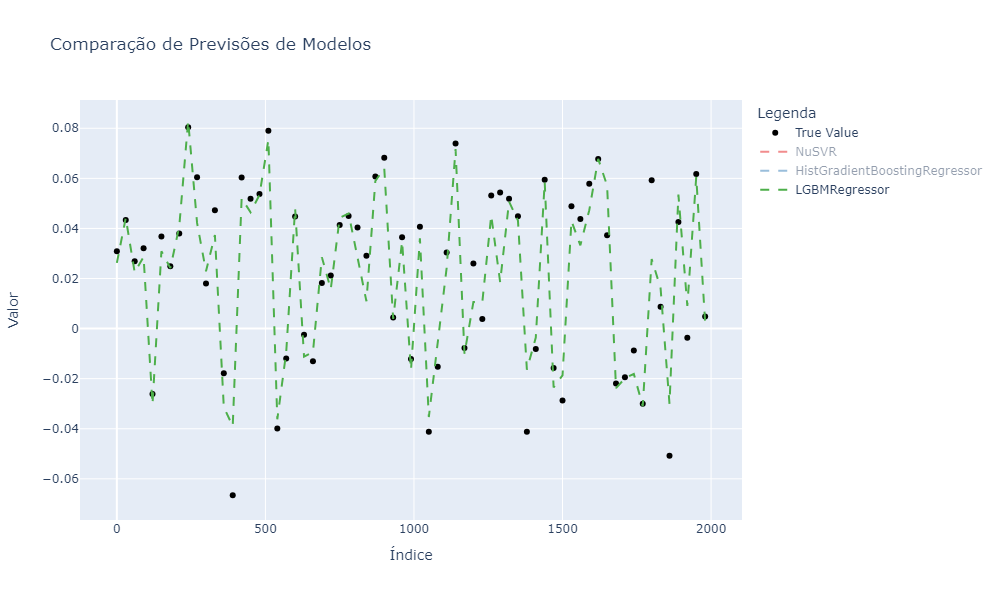
\includegraphics[width=1\linewidth]{LGBMRegressor_func.png}
    \caption{Função da LightGBMRegressor}
    \label{fig:LGBM_Func}
\end{figure}

\begin{figure}[H]
    \centering
    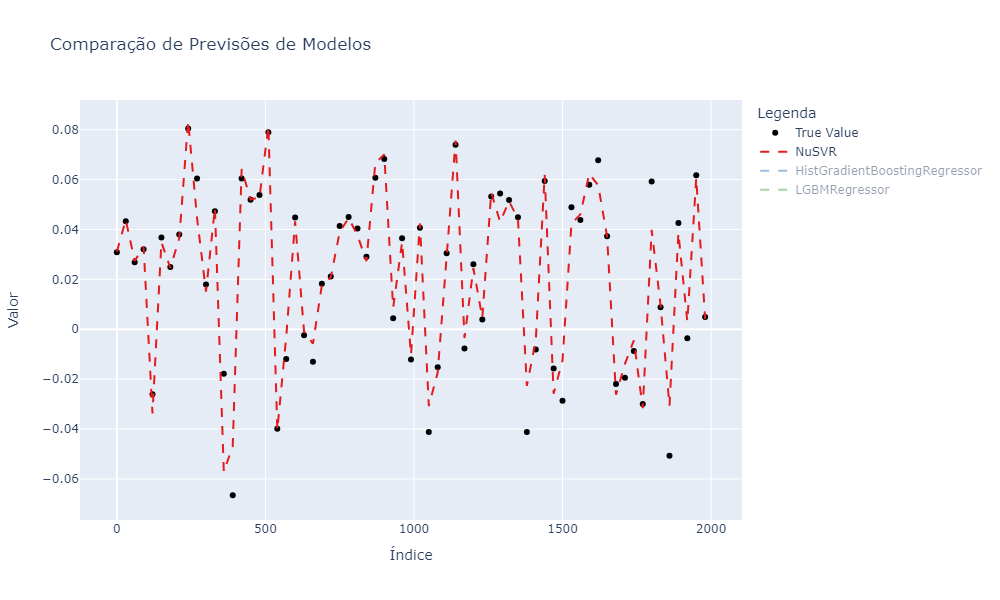
\includegraphics[width=1\linewidth]{NuSVR_Func.png}
    \caption{Função da NuSVR}
    \label{fig:NuSVR_Func}
\end{figure}

\begin{figure}[H]
    \centering
    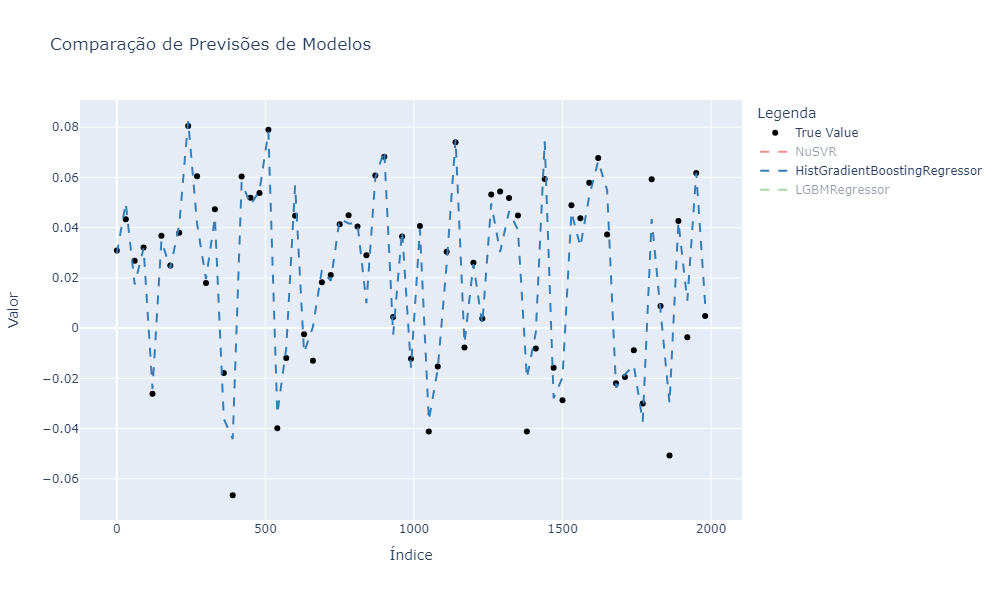
\includegraphics[width=1\linewidth]{HistGradientBoostingRegressor.png}
    \caption{Função da HistGradientBoostingRegressor}
    \label{fig:HGBR_Func}
\end{figure}

O modelo mais promissor de acordo com esses resultados parece ser o LGBM e para chegar a uma conclusão é necessária uma discussão mais aprofundada sobre esses dados.


\subsection{Algoritmo Genético}

Para o algoritmo genético foram utilizados dois métodos e portanto resultou em alguns resultados diferentes, o primeiro método foi o mais pesado, pois utiliza de várias equações e retorna vários fitness, enquanto o segundo método utiliza várias equações para um fitness só.

Os resultados do primeiro foram:
\begin{figure}[H]
    \centering
    \includegraphics[width=1\linewidth]{multivariaveis_fitness_grafico.jpg}
    \caption{Gráfico de fitness para AG multivariaveis}
    \label{fig:multi_grafico}
\end{figure}

Nesse gráfico é possivel verificar que o comportamento do fitness em relação as gerações foi o esperado. Porém tem alguns pontos impotantes sobre esses dados, não foi feito nenhum cross entropy, portanto pode existir overfitting.

As medidas de erro foram:
\begin{figure}[H]
    \centering
    \includegraphics[width=1\linewidth]{multivariaveis_fitness.jpg}
    \caption{Valores de erro do AG de multivariáveis}
    \label{fig:multi_fit}
\end{figure}

Além de ficar evidente os valores das medidas de erro, é possivel também visualizar os valores dos parâmetros utilizados.

E para o AG padrão foram utilizadas 8000 equações por geração com 2000 soluções por geração e 400 separadas para elitização, com 3000 gerações por k fold em k = 5.

O gráfico do fitness em relação as gerações foi:
\begin{figure}[H]
    \centering
    \includegraphics[width=1\linewidth]{fitness_80_20.jpg}
    \caption{Gráfico de fitness para AG multivariaveis}
    \label{fig:80_20_Grafico}
\end{figure}

Além disso as medidas de erro foram:
\begin{figure}[H]
    \centering
    \includegraphics[width=1\linewidth]{fitness_80_20_Medidas_de_erro.jpg}
    \caption{Medidas de erro para o Algoritmo Genético}
    \label{fig:fitness_80_20_Medidas_de_erro}
\end{figure}

Isso apresenta alguns resultados valiosos, porém com um mape muito alto, e nesse caso quanto menor melhor.

\section{Discussões}
Ao avaliar o desempenho dos modelos Nu Support Vector Regression (NuSVR), LightGBMRegressor (LGBM) e Histogram-Based Gradient Boosting Regression (HistGradientBoostingRegressor), observa-se que o NuSVR está superando os outros dois em termos de performance. No entanto, este modelo só atinge tais resultados quando utiliza cerca de 90\% dos dados como Vetores de Suporte, o que sugere um possível sobreajuste (overfitting). Para mitigar este problema, é recomendável reduzir a proporção de dados utilizados como Vetores de Suporte, visando melhorar a capacidade de generalização do modelo.

Por outro lado, tanto o HistGradientBoostingRegressor quanto o NuSVR demonstram tendência ao sobreajuste em suas atuais configurações.

Em contraste, o LightGBMRegressor se destaca por apresentar uma maior resistência ao overfitting, mantendo um desempenho mais estável e generalizável. Este comportamento sugere que o LightGBMRegressor pode ser uma escolha mais robusta em cenários onde a generalização é crítica, enquanto os outros modelos requerem ajustes mais finos para evitar sobreajuste. Outro ponto importante que reforça a ideia do LightGBMRegressor ser mais geral é ter as medidas de erro mais altas, o que implica que estão ligeiramente mais distantes dos pontos de objetivo, o que significa uma menor aproximação e maior generalização e isso fica ainda mais claro com a visualização da função na imagem \ref{fig:LGBM_Func}.

Ficam claros alguns pontos também como a diferença entre os métodos mais simples como regressão linear e árvores de decisão para regressão em relação aos modelos escolhidos, isso é muito proveitoso em relação á otimização e busca de resultados realmente eficientes.

\subsection{Algoritmo Genético}

Com os resultados apresentados em relação ao algoritmo genético, algumas informações são importantes, primeiro é que o treino utilizando pygad foi do tipo $\lambda X_1 + \lambda X_2 + ... + \lambda X_n = Y$, portanto não tiveram mudanças nas operações realizadas na equação e sim nos valores de lambda.

Os valores de lambda foram apresentados e ao aplica-los em qualquer linha da base de dados, deveria retornar um stab semelhante. (Para os dois métodos de AG utilizados)

Além disso, é possivel fazer uma comparação dos modelos de AG e suas métricas de erro.

O resultado foi que o MSE MAE e RMSE foi melhor no algoritmo genético, porém o MAPE ficou muito grande para os dois casos.

Olhando pelo grafico e pelos resultados de erro o AG multivariado performou melhor, porém demorou muito mais para rodar, ou seja, seria muito custoso para rodar para as 8000 equações e fazer cross validation assim como o outro método.

O problema do multivariável é que apenas 10 funções das 10000 foram utilizadas como base para criação da equação.

Enquanto isso o AG feito por ultimo usou 80\% das equações totais.

Também seria interessante fazer algumas aplicações a mais como colocar maior número de solução por população, mas isso exige demais de um computador, que mesmo rodando em cuda com uma 3050 estava devagar.

Todo o momento que aumentou o numero de solução por população, foi notavel um maior desempenho em relação a fitness.

O que fica claro entre esses modelos é que o que rodou para mais equações teve um resultado geral pior, porém nele também poderiam ter sido feitas alterações e aumentar a quantidade de solução por população, quantidade de gerações e etc... E consequentemente retornar resultados mais eficientes.


\section{Conclusão}

Conclui-se que, embora o modelo NuSVR apresente desempenho superior em determinadas condições, sua eficácia está fortemente atrelada a uma configuração que pode levar ao sobreajuste, comprometendo sua capacidade de generalização. Da mesma forma, o HistGradientBoostingRegressor também exibe sinais de overfitting, necessitando de ajustes adicionais para melhorar sua robustez. Em contrapartida, o LightGBMRegressor demonstrou maior resistência ao overfitting, destacando-se como uma opção mais confiável para modelos de regressão que exigem estabilidade e precisão em ambientes de dados variados. Portanto, a escolha do modelo ideal deve considerar não apenas o desempenho imediato, mas também a capacidade de generalização, com o LightGBMRegressor emergindo como uma alternativa sólida em contextos onde a generalização é uma prioridade.

Em relação aos algoritmos genéticos fica possivel concluir que foram encontrados ótimos MAE, MSE e RMSE, porém um MAPE ruim. E além disso o gráfico de fitness da AG multivariavel ficou mais como o desejado de acordo com a literatura, e apresentou um MAPE melhor, portanto o indicado seria aprofundar um pouco no conteúdo desse tipo de AG e melhorar o código para resultados mais otimizados e precisos.

\begin{thebibliography}{1}
    \bibitem{Deng2023}
    Y. Deng, K. K. Cao, W. Hu \textit{et al.}, "Harmonized and Open Energy Dataset for Modeling a Highly Renewable Brazilian Power System," \textit{Scientific Data}, vol. 10, no. 103, 2023, doi: 10.1038/s41597-023-01992-9.

    \bibitem{Brown2018}
    T. Brown, J. Hörsch, and D. Schlachtberger, "PyPSA: Python for Power System Analysis," \textit{Journal of Open Research Software}, vol. 6, no. 1, 2018, arXiv:1707.09913, doi: 10.5334/jors.188.

    \bibitem{SAP2024}
    SAP Insights, "The Smart Grid: How AI is Powering Today’s Energy Technologies," Available: \textit{SAP Insights}, Accessed: Jul. 11, 2024.

    \bibitem{Satu2024}
    Md. Satu and Md. Imran Khan, "Machine Learning Approaches To Predict The Stability of Smart Grid," 2024, doi: 10.21203/rs.3.rs-3866218/v1.

    \bibitem{Deng2021}
    Y. Deng, "PyPSA-Brazil: A Free and Open Model of the Brazilian Electrical System," in \textit{Energy Proceedings}, 2021.

    \bibitem{Zheng2022}
    X. Zheng, N. Xu, L. Trinh \textit{et al.}, "A multi-scale time-series dataset with benchmark for machine learning in decarbonized energy grids," \textit{Scientific Data}, vol. 9, no. 359, 2022, doi: 10.1038/s41597-022-01455-7.

    \bibitem{Shi2024}
    Y. Shi, G. Ke, D. Soukhavong, J. Lamb, Q. Meng, T. Finley, T. Wang, W. Chen, W. Ma, Q. Ye, T. Liu, N. Titov, and D. Cortes, "lightgbm: Light Gradient Boosting Machine," R package version 4.5.0.99, 2024. Available: https://github.com/Microsoft/LightGBM.

    \bibitem{Arzamasov2018}
    V. Arzamasov, K. Böhm, and P. Jochem, "Towards Concise Models of Grid Stability," in \textit{2018 IEEE International Conference on Communications, Control, and Computing Technologies for Smart Grids (SmartGridComm)}, Aalborg, Denmark, 2018, pp. 1-6, doi: 10.1109/SmartGridComm.2018.8587498.

    \bibitem{Chen2016}
    T. Chen and C. Guestrin, "XGBoost: A Scalable Tree Boosting System," in \textit{Proceedings of the 22nd ACM SIGKDD International Conference on Knowledge Discovery and Data Mining}, San Francisco, CA, USA, 2016, pp. 785-794, doi: 10.1145/2939672.2939785.

\end{thebibliography}

\end{document}
